

\subsection{Installation des I2P-Routers}
F�r die Nutzung des Invisible Internet Projects ben�tigt man den I2P-Router, der als Proxy f�r verschiedene Anwendungen (Webbrowser, E-Mail Client...) dient und die Weiterleitung der Daten vom und zum I2P-Netz �bernimmt. Der I2P-Router ist eine Java-Applikation und steht unter \href{http://www.i2p2.de}{www.i2p2.de} zum Download bereit.\\

\begin{description}
 \item[Windows:] Als erstes ist ein Java-Runtime-Environment (JRE) zu installieren. Das Installationsprogramm f�r Java gibt auf der Webseite www.java.com\footnote{ \href{http://www.java.com/de/}{http://www.java.com/de/}}. Der Installer m�chte unbedingt die \textit{Ask-Toolbar} f�r alle Browser installieren. Das sollte man deaktivieren, braucht man nicht.\\

 WICHTIG: Der Installer aktiviert auch ein Java-Plugin f�r alle Browser. Dieses Plug-in ist ein Sicherheitsrisiko und muss im Java Control Panel unter \textit{Systemsteuerung - Programme - Java} deaktiviert werden!
\begin{center}
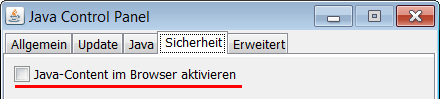
\includegraphics[scale=0.55]{../screenshots/java-ctrl-klein.png}
\end{center}

 Anschlie�end kann der I2P-Router installiert werden. Die Datei \textit{i2pinstall-0.x.y.exe} von der I2P Downloadseite \href{http://www.i2p2.de/download.html}{http://www.i2p2.de/download.html} enth�lt einen kompletten Installer, der nach dem Start alles N�tige einrichtet. Einfach starten und dem Assistenten folgen. Nach der Installation findet man im Startmen� die neue Gruppe \textit{I2P} (Bild \ref{abb:i2pstartwin}).\\
 
  \begin{figure}[htb]
  \begin{center}
  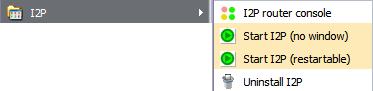
\includegraphics[scale=0.60]{../screenshots/i2p-win.png}
  \caption{I2P im Startmen� von Windows}
  \label{abb:i2pstartwin}
  \end{center}
  \end{figure}

Die beiden Punkte zum Starten von I2P unterscheiden sich nur gering. Im ersten Fall hat man keine st�rende Konsole auf dem Desktop. \textit{I2P router console} �ffnet den Webbrowser, um den Router zu konfigurieren oder abzuschalten mit der Adresse \href{http://localhost:7657}{http://localhost:7657}.
